% Unofficial UChicago CS Poster Template
% v1.1.0 released September 8, 2022
% https://github.com/k4rtik/uchicago-poster
% a fork of https://github.com/anishathalye/gemini

\documentclass[final]{beamer}

% ====================
% Packages
% ====================

\usepackage[T1]{fontenc}
\usepackage{lmodern}
\usepackage[size=custom,width=120,height=72,scale=1.0]{beamerposter}
\usetheme{gemini}
\usecolortheme{uchicago}
\usepackage{graphicx}
\usepackage{booktabs}
\usepackage{bm}
\usepackage[ruled]{algorithm2e}
%\usepackage{enumitem}
\usepackage{doi}
\usepackage[numbers]{natbib}
\usepackage[patch=none]{microtype}
\usepackage{arydshln}
\usepackage{tikz}
\usepackage{pgfplots}
\pgfplotsset{compat=1.18}
\usepackage{anyfontsize}
\usepackage{subcaption}
\usepackage{wrapfig}
\usepackage{outlines}
\usetikzlibrary{arrows,shapes}

\pdfstringdefDisableCommands{%
\def\translate#1{#1}%
}

% ====================
% Lengths
% ====================

% If you have N columns, choose \sepwidth and \colwidth such that
% (N+1)*\sepwidth + N*\colwidth = \paperwidth
\newlength{\sepwidth}
\newlength{\colwidth}
\setlength{\sepwidth}{0.025\paperwidth}
\setlength{\colwidth}{0.3\paperwidth}

\newcommand{\separatorcolumn}{\begin{column}{\sepwidth}\end{column}}

% ====================
% Title
% ====================

\title{Walk Less and Only Down Smooth Valleys}

\author{Thomas Brink (tbrink@stanford.edu) \and Julian Cooper (jelc@stanford.edu) \and Quinn Hollister (bh9vw@stanford.edu)}


% ====================
% Footer (optional)
% ====================

%\footercontent{
%  \href{https://www.example.com}{https://www.example.com} \hfill
%  CS229 Poster session, Stanford University --- XYZ-1234 \hfill
%  \href{mailto:alyssa.p.hacker@example.com}{alyssa.p.hacker@example.com}}
% (can be left out to remove footer)

% ====================
% Logo (optional)
% ====================

% use this to include logos on the left and/or right side of the header:
% \logoright{\includegraphics[height=7cm]{logo1.pdf}}


% ====================
% Body
% ====================

\begin{document}
\addtobeamertemplate{headline}{}
{
    \begin{tikzpicture}[remember picture,overlay]
     % \node [anchor=north west, inner sep=3cm] at ([xshift=0.0cm,yshift=1.0cm]current page.north west)
      %{\includegraphics[height=5.0cm]{logos/uc-logo-white.eps}}; % also try shield-white.eps
      \node [anchor=north east, inner sep=2.3cm] at ([xshift=0.0cm,yshift=2.5cm]current page.north east)
      {
\includegraphics[height=7.5cm]{stanford.png}};
    \end{tikzpicture}
}


\begin{frame}[t]
\vfill
\begin{block}{\large Problem \& Motivation}
  % \centering
  Transfer learning has become a valuable tool for handling a variety of downstream NLP tasks given a single generic pre-trained model. Since most of the downstream tasks are specialized, quality training data is a scarce resource, making training large models from scratch very difficult. 
  In this project, we investigate how the performance of a pre-trained BERT encoder model changes for three different downstream prediction tasks when we include (i) regularization in our fine-tuning loss function and parameter (SMART by Jiang et al. \cite{smart}), (ii) multitask learning on fine-tuning datasets \cite{MTL}, and (iii) introduce relational layers that exploit similarity between tasks \cite{MTL}. Our default minBERT model is pre-trained using two unsupervised tasks on Wikipedia articles: masked language modeling and next sentence prediction. For fine-tuning on downstream prediction tasks, we use the \textit{Stanford Sentiment Treebank} (SST, 11,855 single sentence reviews), \textit{Quora} (400,000 question pairs), and \textit{SemEval STS Benchmark} (STS, 8,628 sentence pairs) datasets. 
  % We find that SMART prevents overfitting that is common in fine-tuning BERT models to downstream tasks when constrained by the size of the particular fine-tuning dataset. Also, we learn this adversarial regularization is less effective when combined with multi-task learning in a rich data environment. Finally, we observe that there is value in 

\end{block}

% \begin{frame}[t]
\begin{columns}[t]
\separatorcolumn

\begin{column}{\colwidth}

  \begin{block}{Extension 1: SMART Regularization}
            
Many fine-tuning routines suffer from overfitting, which leads to poor performance on test sets of downstream prediction tasks. To address this, we implement the SMART regularization technique by Jiang et al. \cite{smart}.

\begin{enumerate}
    \item \textbf{Adversarial regularization}: The desired property is that when the input $x$ is perturbed by a small amount, the output should not change much. To achieve this, Jiang et al. \cite{smart} optimize loss $\mathcal{F}(\theta)$ using: $\min_{\theta} \mathcal{F}(\theta) = \mathcal{L}(\theta) + \lambda_{s}\mathcal{R}_{s}(\theta)$, where
    \begin{align*}
    \mathcal{L}(\theta) & = \frac{1}{n} \sum_{i=1}^{n} l(f(x_{i};\theta), y_{i}) && \text{regular loss function} \\
    \mathcal{R}_{s}(\theta) & = \frac{1}{n} \sum_{i=1}^{n} \max_{\lVert \Tilde{x_{i}} - x_{i} \rVert_{p \leq \epsilon}} l_{s}\left(f(\Tilde{x_{i}}; \theta), f(x_{i}; \theta)\right) && \text{regularization term}\\
    l_{s}(P, Q) & = \mathcal{D}_{KL}(P \lVert Q) + \mathcal{D}_{KL}(Q \lVert P) && \text{symmetric KL-divergence}
    \end{align*} \newline

    \item \textbf{Bregman proximal point optimization}: To prevent aggressive updating, the optimization routine is changed so that we introduce a trust-region-type regularization at each iteration, so we only update the model within a small neighborhood of the previous iterate. Specifically, we update parameters $\theta$ by $\theta_{t+1} = \text{argmin}_{\theta} \mathcal{F}(\theta) + \mu \mathcal{D}_{Breg}(\theta, \Tilde{\theta_{t}})$, where
    \begin{align*}
    \mathcal{D}_{Breg}(\theta, \Tilde{\theta_{t}}) & = \frac{1}{n} \sum_{i=1}^{n} l_{s} \left( f(x_{i}; \theta), f(x_{i}; \Tilde{\theta_{t}}) \right) && \text{Bregman divergence} \\
    \Tilde{\theta}_{t} & = (1 - \beta)\theta_{t} + \beta \Tilde{\theta}_{t-1} && \text{regularized update step}
    \end{align*}
\end{enumerate}

\textbf{Customizations}. Although we were mostly able to follow the authors' algorithm, we needed to customize the algorithm to handle dropout. To do this, we remove dropout (switch to eval mode) when evaluating the adversarial loss within the training block. This allowed us to achieve the desired asymptotic behaviour with respect to our $\epsilon$ parameter. We publish psuedocode for our revised algorithm in the writeup appendix.

We decided not to invest time doing a large hyperparameter grid search for this project since we had access to suggested values from the original paper and limited compute resources. However, we did vary our regularization weight term $\lambda = \{0.01, 0.1, 1, 5, 10, 100\}$ for a small number of iterations to confirm regularization was being applied at the right order of magnitude.


% \begin{algorithm}
% \KwData{$\hat{f}$: model, $\{x_{i}\}_{1}^{Q}$: model embeddings, $\{z_{j}\}_{1}^{B}$: batch inputs, $\sigma^{2}$: variance of noise, $\eta = 10^{-3}$: learning rate for adversarial update, $\epsilon = 10^{-5}$: max perturbation.}
% \Begin{
%     $\hat{f}$ set to eval mode \\
%     $y_{j} \longleftarrow \hat{f}(z_{j}, x)$ \\
%     \For{$ x_{i} \in \mathcal{Q}$}{
%         $\Tilde{x}_{i} \longleftarrow x_{i} + \nu_{i}$    with $\nu_{i} \sim \mathcal{N}(\mathbf{0}, \sigma^{2} \mathbf{I})$
%     } 
%     \For{$ y_{j} \in \mathcal{B}$}{
%         $\Tilde{h}_{j} \longleftarrow \nabla_{\tilde{x}} l_{s}(y, \hat{f}(z_{j}, x))$
%     }
%     $\Tilde{g}_{i} \longleftarrow \left(\frac{1}{|\mathcal{B}|} \sum_{i} \Tilde{h}_{j} \right)\left( \lVert    \frac{1}{|\mathcal{B}|} \sum_{i} \Tilde{h}_{j} \rVert_{\infty}\right)^{-1}$ \\
%     \For{$x_{i} \in \mathcal{Q}$}{
%         $\Tilde{x}_{i} \longleftarrow \mathcal{P}_{\lVert \Tilde{x}_{i} + \eta \Tilde{g}_{i} - x_{i}\rVert \leq \epsilon} \left( \Tilde{x}_{i} + \eta \Tilde{g}_{i} \right)$
%     }
%     $y^{\text{adv}}_{j} \longleftarrow \hat{f}(z_{j}, \Tilde{x})$ \\
%     $\mathcal{L}_{\text{adv}, \text{classification}} \longleftarrow \frac{1}{|\mathcal{B}|} \sum_{j \in \mathcal{B}} \mathcal{D}_{KL}( y_{j} || y^{\text{adv}}_{j}) + \mathcal{D}_{KL}( y^{\text{adv}}_{j} || y_{j})$ \\
%     $\mathcal{L}_{\text{adv}, \text{regression}} \longleftarrow \frac{1}{| \mathcal{B} |} \sum_{j \in \mathcal{B}} \lVert y_{j} - y^{\text{adv}}_{j} \rVert^{2}$ \\
%     $\hat{f}$ set to train mode
% }
% \caption{SMART: Adversarial Loss Calculation}
% \label{alg: smart-adv}
% \end{algorithm}

  \end{block}

\begin{alertblock}{\small Discussion and takeaways}

\begin{itemize}

 \item Benefits of SMART regularization are most pronounced when the fine-tuning dataset is small or ill-balanced. Areas of the feature space that are sparsely covered in such a dataset will tend to create sharp decision boundaries that may not be generalizable, and hence perform poorly on out-of-sample tests.
 \item However, incremental benefits of regularization decrease with the size of data used and regularization may even restrict learning too much in this setting.

\end{itemize}

\end{alertblock}

\end{column}

\separatorcolumn

\begin{column}{\colwidth}

  \begin{block}{Extensions 2-3: Multitask Learning}

    Fine-tuning the default BERT model does not generalize well to other downstream prediction tasks. To design an approach that is generalizable across different tasks, we implement two multi-task learning routines. 
    
    \begin{enumerate}%[(a)]%[label=(\alph*)]
      \item \textbf{Round-Robin Multitask Fine-Tuning}
      \begin{itemize}
      \normalsize
          \item Equally-weighted round-robin: train on all prediction tasks while balancing data.
          \item Additional pretraining: exploit rich paraphrase data through additional pretraining.
          \item Interleaved fine-tuning: batch-adjusted task-specific network on top of BERT.
          \vspace{-0.3cm}
      \end{itemize}
          \begin{figure}[H]
     \centering
     \begin{subfigure}[b]{0.485\textwidth}
         \centering
        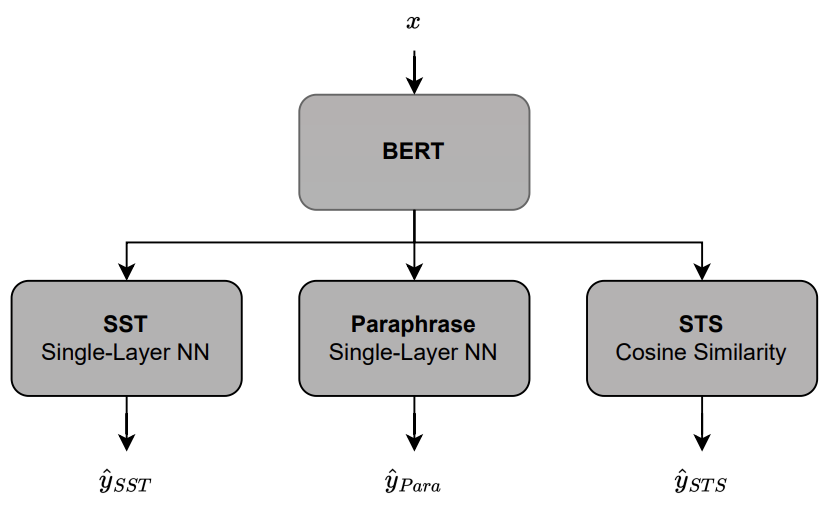
\includegraphics[width=0.9\textwidth]{writeup/round-robin.png}
         \caption{}
         %\label{fig:y equals x}
     \end{subfigure}
     \begin{subfigure}[b]{0.485\textwidth}
        \centering
        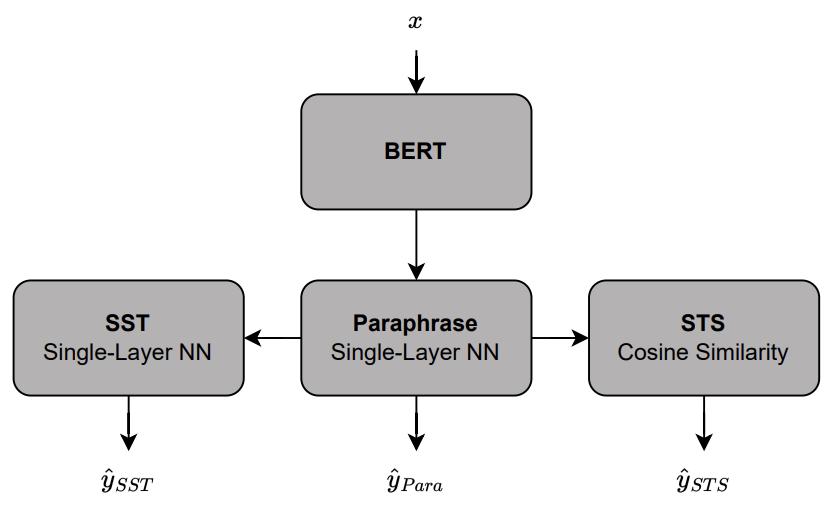
\includegraphics[width=0.9\textwidth]{writeup/add-pretrain.png}
         \caption{}
         %\label{fig:three sin x}
     \end{subfigure}
\caption{Model architectures for equally-weighted round-robin and interleaved fine-tuning in (a) and additional pretraining in (b).} %cycle life}
\label{fig:birds}
\end{figure} 
      
      \item \textbf{Rich Relational Layer Combining Similar Tasks} 
      \begin{itemize}
      \normalsize
          \item Capture similarities across tasks to synergize joint performance.
          \item Share relational layer between rich paraphrase data and STS data on top of BERT.
      \end{itemize}  
      \begin{figure}[h]
    \centering
    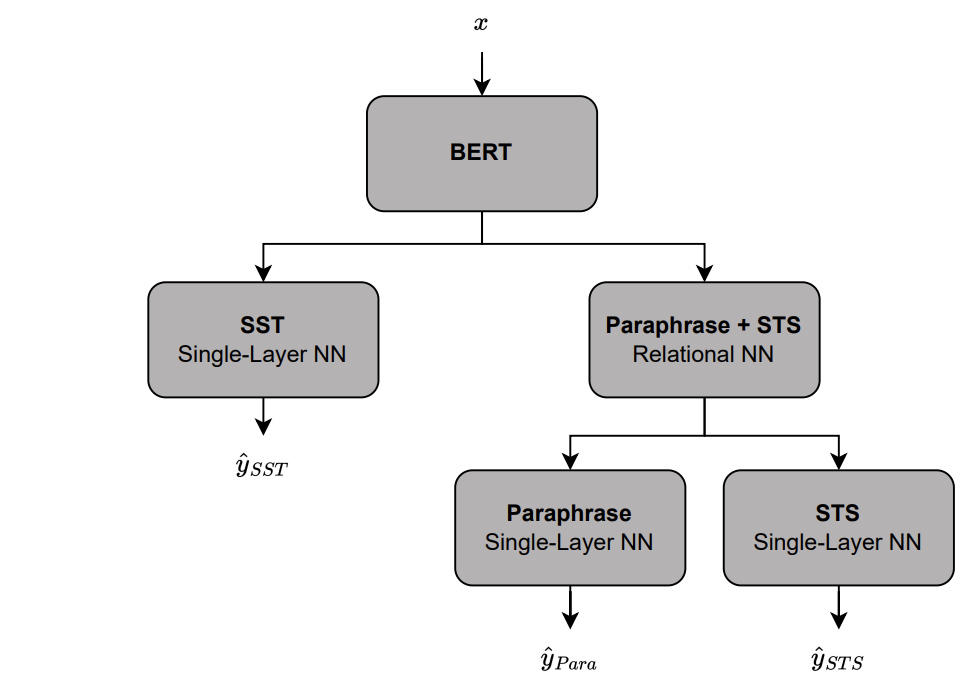
\includegraphics[width=0.485\textwidth]{writeup/rich-rel.png}
    \caption{Network architecture for the rich relational approach.}
\end{figure}
    \end{enumerate}
    %Noticing that the paraphrase and STS datasets exhibit strong similarities, we design a multi-task learning approach that can capture rich relationships between tasks. Its main features include:
  \end{block}
\vspace{-1.2cm}
  \begin{alertblock}{\small Discussion and takeaways}
  \begin{outline}
      \1  The benefit of introducing more data has proven to be greater than the potential risk of an imbalanced multitask fine-tuning procedure.
      \1  For all data-rich models, SST accuracy slightly dropped. This is likely caused by the added Quora data being orthogonal to or disrupting the sentiment task.

  \end{outline}
     
  \end{alertblock}
\end{column}

\separatorcolumn

\begin{column}{\colwidth}

\begin{block}{Experiments \& Analysis}
Table \ref{tab: single} compares the dev accuracy of our default model (pretrain and finetune) with benchmarks provided in the handout for the single-task classifier. Our results are all close to the benchmarks which gives us confidence in the `correctness' of our default implementation. 
\begin{table}[h]
\footnotesize
\centering
\caption{\textit{Dev accuracy of baseline BERT models (pretrain and fine-tune) vs. benchmarks for single-task classifier and runtimes per training epoch on a Google Colab GPU.}}
\begin{tabular}{|l|ccc|ccc|}
\hline
  & \multicolumn{3}{c|}{\textbf{Sentiment (SST)}} & \multicolumn{3}{c|}{\textbf{Sentiment (CFIMDB)}} \\ \hline
\textbf{Model type}       & Accuracy       & Benchmark & Runtime (s)          & Accuracy        & Benchmark & Runtime (s)           \\ \hline
Pretrain default & 0.393           & 0.390 (0.007) & 30    & 0.788            & 0.780 (0.002)  & 45     \\
Fine-tune default & 0.522           & 0.515 (0.004) & 120    & 0.963            & 0.966 (0.007) & 150      \\ \hline
\end{tabular}
\label{tab: single}
\end{table}
% \vspace{-0.5cm}

Table \ref{tab: multi} gives the dev performance for all proposed model approaches on the SST, Quora, and STS tasks. We include three non-multitask models; the baseline models from Table \ref{tab: single} (i.e., BERT and fine-tuned SST) and an SST-fine-tuned model with SMART. Furthermore, we evaluate various multitask learning approaches combining SMART, round-robin, and the rich relational layer model.  

% Table \ref{tab: multi} compares dev accuracies of our default implementation (treated as our baseline from now on) with the different model extensions. For the milestone, we had implemented batch-level round-robin and SMART regularization extensions, which both independently improved our model's overall performance. In particular, we saw improvements in the paraphrase and similarity tasks. Our best milestone result came from combining both extensions (rrobin+smart), although this does significantly increase computation time.

\begin{table}[h]
\footnotesize
\centering
\caption{\textit{Dev set accuracies of single- and multitask models on three fine-tune tasks. The models are divided into three groups; (i) single-task approaches, (ii) small-scale (equally-weighted batches) approaches, and (iii) large-scale rich (relational) approaches. The best model for each task is bolded. Runtimes are given in seconds per training epoch on an AWS EC2 instance.}}
\begin{tabular}{|l|cccc|} \hline
& \multicolumn{1}{c}{\textbf{Sentiment (SST)}} & \multicolumn{1}{c}{\textbf{Paraphrase (Quora)}} & \multicolumn{1}{c}{\textbf{Similarity (STS)}} &  \\ \hline
\textbf{Model type} & Accuracy & Accuracy & Correlation & Runtime (s) \\ \hline
Pretrain default      & 0.396         & 0.380            & 0.019 & 9          \\
Fine-tune default      & 0.525        & 0.522           & 0.240 &  25         \\ 
Fine-tune smart        & 0.520             & 0.501           & 0.382 & 161          \\ \hdashline
Fine-tune rrobin       & 0.524            & 0.726            & 0.583   & 67        \\
Fine-tune rrobin+smart & \textbf{0.532}              & 0.741            & 0.680 & 464          \\ \hdashline
Fine-tune rrobin-pre+smart & 0.519          & 0.851           & 0.690 & 3,037         \\
Fine-tune rrobin-full & 0.498          & 0.863           & 0.762 & 1,420         \\ 
Fine-tune rrobin-full+smart & 0.485          & 0.850           & 0.714 & 4,549         \\
Fine-tune rrobin-full+rlayer & 0.501     & \textbf{0.867}         & \textbf{0.802}    & 1,550                 \\ \hline
\end{tabular}
\label{tab: multi}
\end{table}

SMART performs best out of the single-task models, achieving the highest STS score. However, unsurprisingly, all multitask models easily beat these single-task baselines in terms of paraphrase and STS scores. Out of the multitask models that only use a limited portion of the available data, the SMART implementation again performs best, especially in terms of STS score. When making use of the entire Quora data, we can see that paraphrase accuracy is significantly boosted, reaching values over 85\%. In this setting, it seems that the added value of SMART vanishes.  

The best model overall is the rich relational interleaved round-robin model, which achieves test set performances of 0.503 (SST), 0.865 (paraphrase), and 0.789 (STS).  In terms of runtime, SMART is most costly, especially when used in combination with richer data.
\vspace{-0.4cm}
% For the final report, we added variations of multitask learning that enabled us to use the full Quora dataset. Our first implementation re-used rrobin+smart for fine-tuning but also added a "pretraining" step for the left over Quroa data. This further improved on our milestone results but came with a significant time cost. Our second implementation varied batch size between datasets for each iteration (rrobin-full). This was our best result overall and balanced usage of data, with balanced multitask learning and regularization. {\color{red}update required}

% Note, round-robin with variable batch size did not improve with SMART regularization (rrobin-full+smart). We provide a hypothesis for why this was the case in the analysis section.
\end{block}
    \begin{alertblock}{\small Discussion and takeaways}

    \begin{itemize}
    \item Our best model combines multitask learning using varying batch sizes with a rich relational layer between correlated tasks. 
    \item One next step we would like to explore is data transformations that allow for continuous multimodal distributions that might better predict semantic similarity.
    
    \end{itemize}
  \end{alertblock}

\end{column}

\separatorcolumn
\end{columns}
\vfill
\begin{block}

    % \nocite{*}
    \footnotesize{\bibliographystyle{plainnat}\bibliography{poster}}

\end{block}

\end{frame}

\end{document}
@article{pretrain,
  author    = {Chi Sun and
               Xipeng Qiu and
               Yige Xu and
               Xuanjing Huang},
  title     = {How to Fine-Tune {BERT} for Text Classification?},
  journal   = {CoRR},
  volume    = {abs/1905.05583},
  year      = {2019},
  url       = {http://arxiv.org/abs/1905.05583},
  eprinttype = {arXiv},
  eprint    = {1905.05583},
  timestamp = {Tue, 21 Jan 2020 13:18:06 +0100},
  biburl    = {https://dblp.org/rec/journals/corr/abs-1905-05583.bib},
  bibsource = {dblp computer science bibliography, https://dblp.org}
}